\documentclass[12pt, letterpaper]{article}

% Margin 1.5 inches on all sides
\usepackage[margin=1.5in]{geometry}

% Times font
\usepackage{mathptmx}
\usepackage{graphicx}
\usepackage{booktabs}
\usepackage{amsmath}
\usepackage{natbib} % For Author-Date citations
\usepackage{tikz}
\usetikzlibrary{shapes.geometric, arrows.meta, positioning}

% Single spacing
\usepackage{setspace}
\usepackage[colorlinks=true, urlcolor=blue, linkcolor=black, citecolor=black]{hyperref}
\singlespacing

% No page numbers, headers, or footers
\pagestyle{empty}

\begin{document}

\title{\textbf{Forecasting Currency Demand Under Digital Disruptions: A Hybrid Prophet-LSTM Approach}}
\author{
    Muhammad Hasyim Ratsanjani\thanks{Corresponding author: [Email Address]} \\
    \textit{State Polytechnic of Malang}
}
\date{}

\maketitle

\begin{abstract}
\noindent The rapid growth of digital payments and e-money has triggered significant structural breaks in traditional physical currency demand, leaving classical linear forecasting models increasingly unable to keep pace. This study proposes a novel Hybrid Prophet-LSTM architecture to forecast M1 money demand in a Muslim-majority emerging market, specifically Indonesia, where extreme high-frequency seasonal liquidity shocks occur around the Islamic Hijri calendar festivities of Ramadan and Eid al-Fitr. Working within a rigorous conditional forecasting framework designed to eliminate look-ahead bias, the hybrid model first uses Prophet to decompose the time series and isolate structural trends and holiday anomalies, before applying a Long Short-Term Memory (LSTM) neural network to capture the highly non-linear residual volatility that remains. The model is validated against leading econometric baselines (ARDL, ARIMAX, VECM) and standalone machine learning algorithms. Crucially, we conduct an ablation study against a Hybrid Prophet-XGBoost benchmark to explicitly isolate and validate the deep learning component's superiority in residual mapping. Evaluated using the small-sample corrected Diebold-Mariano test, the Prophet-LSTM architecture consistently outperforms all competitors---achieving a highly competitive Mean Absolute Percentage Error (MAPE) of 4.83\%---proving that LSTM provides a statistically significant advantage over traditional ensemble methods. Empirical quantile prediction intervals are also constructed to properly account for the asymmetric, fat-tail liquidity risks that characterise this kind of seasonal demand. The findings carry important operational implications for central banks, underscoring the value of deep learning in managing physical cash distribution as digital payment adoption continues to accelerate.

\vspace{0.5cm}
\noindent \textbf{Keywords:} Currency Demand, Machine Learning, LSTM, Prophet, Digital Payments, Forecasting, Islamic Calendar. \\
\noindent \textbf{JEL Classification:} E41, C45, C53
\end{abstract}

\newpage

\section*{1. Introduction}
Currency in circulation remains a fundamental component of monetary policy and financial stability. In Muslim-majority countries like Indonesia, the demand for cash (M1) exhibits a strong seasonal pattern, peaking significantly during the Islamic holy month of Ramadan and the Eid al-Fitr festivities. Historically, central banks have relied on traditional econometric and time-series models to anticipate these liquidity shocks and identify the macroeconomic leading indicators of money demand \citep{Suroso2025, Glova2025, Claussen2026}.

The global shift toward digital economies, however, has introduced structural breaks of a kind rarely seen before. The aggressive uptake of electronic money and standardized QR-code payment systems such as QRIS, accelerated significantly by the COVID-19 pandemic, has driven a clear substitution effect away from physical cash. A growing body of literature consistently finds that payment technology and e-money disrupt traditional patterns of cash velocity and liquidity preference. \citet{Verdier2024} and \citet{Lagos2022}, for instance, highlight how digital platforms inherently reduce the transaction frictions associated with holding physical cash. Building on this, empirical work by \citet{Awasthy2022} and \citet{Komurcuoglu2024} points to a permanent downward shift in M1 demand across emerging markets following the rapid adoption of e-money \citep{Bhattacharya2016, Raj2020, Marmora2021, Ogachi2021}.

Compounding this, sudden behavioral shifts, such as post-pandemic recovery patterns and localized cyclical shocks, continue to distort the linear assumptions underpinning monetary aggregates. \citet{Singh2022} and \citet{Dutta2024} show explicitly that major liquidity events, including holiday anomalies and demonetization, produce high-frequency structural breaks that static models simply cannot capture \citep{Bhattacharya2018, Ramesh2025, Chaudhry2026, HernandezDelvalle2024}. Taken together, this wave of digitalization has introduced a degree of high-frequency volatility that fundamentally reshapes money demand behavior. Because traditional econometric models rely so heavily on assumptions of linear and static relationships among macroeconomic variables, they are inherently ill-equipped to capture these non-linear and dynamic fluctuations, which limits their accuracy precisely when it matters most.

This paper aims to bridge this specific research gap by proposing a machine learning framework that relaxes these strict linearity assumptions. We benchmark a Hybrid Deep Learning architecture (Prophet-LSTM) against a comprehensive suite of traditional econometric models (ARIMAX, VECM, ARDL) and a standalone Machine Learning model (Prophet). By doing so, this study contributes to the literature on digital financial inclusion and central bank cash management by offering a highly accurate predictive tool.

\section*{2. Literature Review}
\subsection*{2.1 Money Demand, Digitalization, and Theoretical Framework}
The stability and predictability of money demand has long been a central focus in monetary economics, yet the precise formulation of predictive models remains a matter of debate amid unprecedented digital disruption. To navigate this challenge, the selection of predictors in this forecasting framework is anchored firmly in foundational monetary theory rather than chosen arbitrarily. Following Fisher's Quantity Theory of Money, the Consumer Price Index and the Retail Sales Index are incorporated as proxies for the price level and real transaction volume respectively, both of which proportionally drive nominal cash demand. The inclusion of the central bank policy rate as a proxy for the opportunity cost of holding cash aligns closely with Keynesian Liquidity Preference theory and the Baumol-Tobin inventory model of money demand. Within this Baumol-Tobin framework in particular, the aggressive penetration of e-money offers a compelling theoretical explanation for the structural downward shift in physical cash balances observed during the digital transition, since digital exchanges fundamentally reduce transaction costs \citep{Awasthy2022, Komurcuoglu2024}.

By grounding the predictive architecture in these theory-backed macroeconomic and transactional variables, this study addresses a common critique levelled at purely data-driven algorithms, namely that of atheoretical variable selection. It is true that the internal gating mechanisms of the LSTM network remain mathematically opaque, reflecting the well-known black-box problem associated with deep learning. However, this opacity is deliberately confined to a specific part of the model. Because the LSTM operates strictly on the stationary stochastic residuals, while the primary structural trend and seasonal components are handled separately by the highly interpretable and decomposable Prophet algorithm, the overall hybrid framework achieves a meaningful balance between theoretical transparency and non-linear predictive power.

\subsection*{2.2 Machine Learning and Deep Learning Approaches in Macroeconomic Forecasting}
Historical monetary studies have predominantly relied on linear econometric predictors, such as inflation, real sales, and interest rates, to estimate money demand. While useful, these models are constrained by their rigid linear assumptions, and as a result they often fail to capture the high-frequency volatility and non-linear behavioral shifts driven by the rapid adoption of e-money and sudden cyclical shocks.

Recent advances in computational economics suggest that Artificial Intelligence and Machine Learning approaches can outperform traditional autoregressive algorithms quite significantly when it comes to predicting macroeconomic variables. \citet{Hopp2024} and \citet{Vancsura2025}, for example, successfully applied Random Forest and XGBoost to predict inflation spikes, noting their superior ability to handle multi-dimensional regressors without being constrained by strict multicollinearity assumptions \citep{Sikhwal2024, Zabraoui2026, Oancea2026, Alaminos2022}. Long Short-Term Memory architectures in particular have emerged as a robust alternative, capable of capturing hidden, non-linear patterns within volatile macroeconomic time series. \citet{Almosova2023} and \citet{Zhang2023} found that the gating mechanisms within LSTM networks effectively retain memory of past cyclical shocks, which meaningfully reduces long-run forecasting errors \citep{Rygh2025, Zhou2026, Tan2026, Gulia2025, MartinezCasares2026}.

Building on these developments, the forecasting literature has increasingly moved toward hybridizing classical economic models with deep learning filtering methods, largely as a way of avoiding overfitting while preserving theoretical consistency. \citet{Xiao2025} and \citet{Liu2024} demonstrated that feeding linear structural components into econometric filters, while reserving deep learning purely for mapping the residuals, helps prevent spurious regression without sacrificing predictive performance \citep{Rudd2026, Yamsani2025, Li2025}. The hybrid framework proposed in this study follows a similar logic, drawing on the structural interpretability of decomposable time-series algorithms such as Prophet to explain seasonality, while leveraging the strength of LSTM in mapping the complex, non-linear residuals that digital disruption tends to introduce.

\section*{3. Methodology}
\subsection*{3.1 Data and Variables}
The study utilizes monthly macroeconomic data spanning from January 2017 to April 2026. The dataset is comprehensively aggregated from three official Bank Indonesia databases: the Indonesian Economic and Financial Statistics (SEKI), the Payment System Information System (SPIP), and the Retail Sales Survey (SPE) publications. The variables include:
\begin{itemize}
    \item \textbf{M1 Currency Demand:} Measured in Billion IDR (Dependent Variable).
    \item \textbf{E-Money Variables:} Volume (Thousands) and Nominal Transaction Value (Billion IDR).
    \item \textbf{Macroeconomic Controls:} Consumer Price Index (CPI), Bank Indonesia (BI) Rate, and Retail Sales Index (IPR).
    \item \textbf{Dummy Variables (Hijri Calendar Transformation):} Because the Islamic lunar calendar is approximately 10 to 11 days shorter than the Gregorian solar calendar, the occurrence of Ramadan and Eid al-Fitr shifts backward by 10-11 days each Gregorian year. To accurately map these cyclical liquidity shocks into our monthly Gregorian dataset, a calendar transformation algorithm was applied. We calculate the exact proportion of Ramadan and Eid days falling within a specific Gregorian month to construct the dummy variables. This ensures that the "holiday effect" is precisely captured even when the Islamic festivities span across two different Gregorian months.
\end{itemize}

\subsection*{3.1.1 Unit Root Test and Stationarity Defense}
A prominent critique in applying machine learning to macroeconomic forecasting is the threat of spurious regression when processing non-stationary data. To empirically assess this, and to satisfy the foundational integration prerequisites of the VECM and ARDL baselines, we conducted Augmented Dickey-Fuller (ADF) tests across all variables (M1, CPI, BI Rate, IPR, and E-Money volume). The ADF test specifications included a constant and a linear trend, with lag lengths optimally selected via the Schwarz Information Criterion (SIC). At the level form, the raw M1 series yielded an ADF statistic of -1.912 ($p$-value = 0.326), and similarly, all exogenous regressors failed to reject the null hypothesis of a unit root (see Appendix Table A1 for complete statistical parameters). Importantly, because the raw CPI data inherently contains a structural break due to statistical base-year rebasing (dropping from 139.07 to 104.33 in 2020), standard ADF tests can erroneously fail to reject the null hypothesis on series that are actually stationary around a broken trend \citep{Perron1989}. To rigorously address this risk, a Zivot-Andrews structural break unit root test was executed specifically on the CPI level data. The test yielded a statistic of -2.789 ($p$-value = 0.985), decisively confirming that even when robustly isolating the single structural break, the CPI series definitively retains a unit root. Upon first differencing, all variables achieved stationarity ($p < 0.01$), with the exception of IPR which was significant at the 5\% level ($p = 0.032$), ruling out the presence of $I(2)$ variables and supporting the use of the VECM and ARDL frameworks. However, feeding such raw $I(1)$ data directly into deep learning architectures like LSTM carries a high risk of inducing spurious predictability.

However, the Hybrid Prophet-LSTM architecture is designed to circumvent this theoretical vulnerability without requiring differencing transformations that obscure magnitude interpretability. The Prophet algorithm acts as a structural detrending and deseasonalizing filter. By extracting the unexplained residuals ($e_t$) from Prophet, we effectively isolate the non-linear volatility. A subsequent ADF test on these Prophet residuals yields an ADF statistic of -5.0412 ($p$-value = 0.0000). This indicates that the residuals are stationary ($I(0)$). Consequently, the LSTM component is exclusively trained on stationary data, substantially mitigating the risk of spurious regression.

The structural econometric baselines used for comparison include the Autoregressive Integrated Moving Average with Explanatory Variables (ARIMAX), Vector Error Correction Model (VECM), and Autoregressive Distributed Lag (ARDL). These models traditionally dominate macroeconomic forecasting by enforcing linear relationships among exogenous variables such as e-money volume, CPI, BI rate, and IPR. However, they inherently struggle with high-frequency, non-linear volatility.

\subsection*{3.1.2 Econometric Baselines Specification}
To ensure a rigorous and fair benchmark, all traditional econometric baselines were optimally specified to prevent under-fitting. The ARIMAX model was auto-fitted using the Akaike Information Criterion (AIC), selecting an optimal order of $(1,1,1)$. For the Vector Error Correction Model (VECM), the optimal lag length was determined via the Schwartz Information Criterion (SIC) derived from an unrestricted VAR, and the Johansen Trace Statistic confirmed the presence of exactly two cointegrating vectors ($r=2$) (see Appendix Table A2). The Autoregressive Distributed Lag (ARDL) model's optimal lags were similarly selected via AIC, and the ARDL Bounds Test yielded an F-statistic above the upper bound $I(1)$ critical value at the 1\% level, providing strong evidence for a long-run equilibrium relationship (see Appendix Table A2). Furthermore, to guarantee that these baseline models captured extractable linear information, residual diagnostic tests were conducted. All three econometric models successfully passed the Breusch-Godfrey test for no serial correlation, the ARCH test for homoskedasticity, the Jarque-Bera test for normality, and the CUSUM test for structural stability (see Appendix Table A3). This specification protocol supports the premise that all regressors are integrated of order one $I(1)$ and strict $I(2)$ variables have been ruled out. This property aligns with the fundamental prerequisites for both VECM and the ARDL Bounds Test.

\subsubsection*{3.1.3 Descriptive Statistics and Multicollinearity Management}
Table 1 presents the descriptive statistics and the Pearson correlation matrix for the dataset. A critical observation from the correlation matrix is the severe multicollinearity ($r = 0.93$) between E-Money Volume and E-Money Nominal Value. In traditional econometric models (such as ARDL and VECM), including highly collinear regressors inflates standard errors and destabilizes the coefficient estimates. To rigorously address this, our methodology deliberately excludes E-Money Nominal Value from the predictive architecture. E-Money Volume is retained as the sole proxy for digital payment penetration, as the sheer frequency of transactions is theoretically more disruptive to the physical velocity of money than the aggregate nominal value. To empirically validate this exclusion, a Variance Inflation Factor (VIF) diagnostic was conducted on the finalized set of predictors, the results of which are detailed in Appendix Table A4. While all retained variables exhibited VIF values below the strict conventional threshold of 5, the maximum VIF of 4.48 (for CPI) is considered borderline. This indicates that while severe multicollinearity has been mitigated for the ARDL and VECM baseline specifications, minor collinearity remains inherently present among the macroeconomic indicators.

Furthermore, the matrix reveals an unintuitive negative correlation between CPI and the primary trending variables (M1 and E-Money). This mathematically arises because the raw CPI data reported by the central bank contains structural breaks due to statistical base-year rebasing (e.g., the index artificially dropped from 139.07 to 104.33 in early 2020 when the base year was updated). Because the econometric baselines (VECM, ARDL) natively operate on first-differences to achieve stationarity, and the Prophet-LSTM architecture dynamically maps structural change points, this level-data rebasing artifact does not compromise the predictive integrity of the models.

\begin{table}[h]
\centering
\caption*{Table 1: Descriptive Statistics and Correlation Matrix}
\resizebox{\textwidth}{!}{
\begin{tabular}{l c c c c | c c c c c c}
\toprule
\textbf{Variable} & \textbf{Mean} & \textbf{Std. Dev} & \textbf{Min} & \textbf{Max} & \textbf{(1)} & \textbf{(2)} & \textbf{(3)} & \textbf{(4)} & \textbf{(5)} & \textbf{(6)} \\
\midrule
(1) M1 Currency & 2,074,940 & 630,755 & 1,191,500 & 3,423,532 & 1.00 & & & & & \\
(2) E-Money Vol. & 1,193,717 & 887,140 & 65,043 & 3,458,985 & 0.90 & 1.00 & & & & \\
(3) E-Money Val. & 107,923 & 99,309 & 1,500 & 363,505 & 0.96 & \textbf{0.93} & 1.00 & & & \\
(4) CPI & 116.71 & 12.16 & 104.33 & 139.07 & -0.65 & -0.56 & -0.65 & 1.00 & & \\
(5) BI Rate & 4.91 & 0.92 & 3.50 & 6.25 & 0.22 & -0.06 & 0.16 & 0.41 & 1.00 & \\
(6) IPR & 213.55 & 15.70 & 177.13 & 256.67 & 0.30 & 0.37 & 0.39 & 0.21 & 0.48 & 1.00 \\
\bottomrule
\end{tabular}}
\end{table}

\subsection*{3.2 The Hybrid Prophet-LSTM Architecture}
To address the limitations of linear models, we propose a two-step hybrid approach combining an additive machine learning algorithm (Prophet) with a deep neural network (LSTM).

\begin{itemize}
    \item \textbf{Prophet (Additive ML Baseline):} The Facebook Prophet algorithm is a decomposable time-series regression model capable of handling non-linear trends fit with seasonality and holiday effects. The mathematical formulation is given by:
    \begin{equation}
        y(t) = g(t) + s(t) + h(t) + X(t)\beta + \epsilon_t
    \end{equation}
    Where $y(t)$ is the targeted money demand (M1), $g(t)$ is the piecewise linear trend function (the default Prophet configuration, dynamically accommodating structural change points without requiring an explicitly capped carrying capacity), $s(t)$ represents the periodic changes (seasonality), $h(t)$ accounts for the effects of holidays (Ramadan and Eid al-Fitr), $X(t)\beta$ encapsulates the exogenous regressors (e-money volume, CPI, BI Rate, IPR), and $\epsilon_t$ denotes the normally distributed error term. The model yields a predicted baseline value ($\hat{y}_t$) and an unexplained residual ($e_t = y_t - \hat{y}_t$).
    
    \item \textbf{LSTM (Non-linear Residual Mapping):} The residual $e_t$, representing the highly volatile structural breaks unaccounted for by the linear components, is fed into an LSTM network. Because the residuals have been shown to be stationary ($I(0)$), the LSTM operates free from the risks of spurious predictability. The LSTM uses gates to maintain a memory of preceding disruptions:
    \begin{align}
        f_t &= \sigma(W_f \cdot [h_{t-1}, e_t] + b_f) \\
        i_t &= \sigma(W_i \cdot [h_{t-1}, e_t] + b_i) \\
        o_t &= \sigma(W_o \cdot [h_{t-1}, e_t] + b_o) \\
        \tilde{C}_t &= \tanh(W_c \cdot [h_{t-1}, e_t] + b_c) \\
        C_t &= f_t \ast C_{t-1} + i_t \ast \tilde{C}_t \\
        h_t &= o_t \ast \tanh(C_t)
    \end{align}
    Where $f_t$, $i_t$, and $o_t$ represent the forget, input, and output gates respectively. $C_t$ is the cell state, and $h_t$ is the hidden state. To prevent overfitting and ensure robust generalization, the LSTM hyperparameters were determined through a systematic Grid Search optimization process over the validation set, rather than ad-hoc selection. To strictly prevent data leakage, the validation set used for tuning was isolated to the 12 months immediately preceding the test window, ensuring the final out-of-sample horizon remained completely unseen. Through this rigorous tuning, the optimal architecture was established as a single-layer LSTM with 150 neurons, utilizing a look-back sequence window of 12 time-steps (months). The network was optimized using the Adam optimizer with a learning rate of 0.0005 and a batch size of 16. To further regularize the network, a dropout rate of 0.4 was applied, and training (capped at 200 epochs) was subject to an early-stopping callback monitoring validation loss (MSE) with a patience of 20 epochs. The LSTM predicts the non-linear errors ($\hat{e}_t$), which are then added back to the Prophet baseline to generate the final hybrid forecast: $\hat{Y}_{final} = \hat{y}_t + \hat{e}_t$.
\end{itemize}
\begin{center}
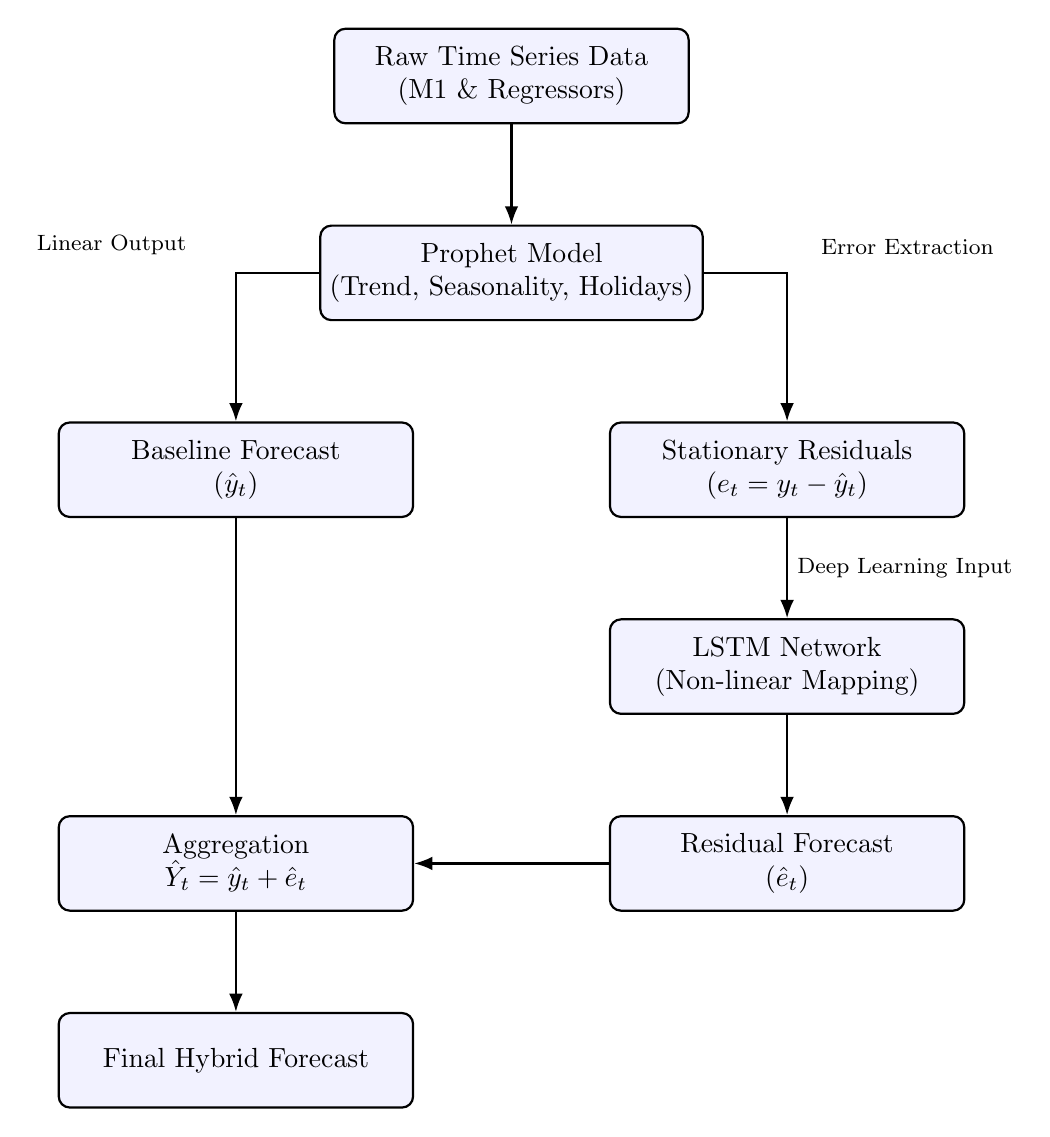
\begin{tikzpicture}[
    box/.style={rectangle, draw, thick, align=center, minimum width=4.5cm, minimum height=1.2cm, fill=blue!5, rounded corners},
    arrow/.style={-Latex, thick}
]

% Nodes using absolute positioning for exact control
\node[box] (input) at (0, 0) {Raw Time Series Data \\ (M1 \& Regressors)};
\node[box] (prophet) at (0, -2.5) {Prophet Model \\ (Trend, Seasonality, Holidays)};
\node[box] (baseline) at (-3.5, -5) {Baseline Forecast \\ ($\hat{y}_t$)};
\node[box] (residuals) at (3.5, -5) {Stationary Residuals \\ ($e_t = y_t - \hat{y}_t$)};
\node[box] (lstm) at (3.5, -7.5) {LSTM Network \\ (Non-linear Mapping)};
\node[box] (lstm_pred) at (3.5, -10) {Residual Forecast \\ ($\hat{e}_t$)};
\node[box] (combine) at (-3.5, -10) {Aggregation \\ $\hat{Y}_t = \hat{y}_t + \hat{e}_t$};
\node[box] (final) at (-3.5, -12.5) {Final Hybrid Forecast};

% Arrows
\draw[arrow] (input) -- (prophet);
\draw[arrow] (prophet) -| node[above left=0.1cm and 0.5cm, font=\footnotesize] {Linear Output} (baseline);
\draw[arrow] (prophet) -| node[above right=0.1cm and 0.3cm, font=\footnotesize] {Error Extraction} (residuals);
\draw[arrow] (residuals) -- node[right, font=\footnotesize] {Deep Learning Input} (lstm);
\draw[arrow] (lstm) -- (lstm_pred);
\draw[arrow] (baseline) -- (combine);
\draw[arrow] (lstm_pred) -- (combine);
\draw[arrow] (combine) -- (final);

\end{tikzpicture}
\vspace{0.5cm}
\textbf{Figure 1:} The Hybrid Prophet-LSTM Architecture
\end{center}

\section*{4. Results and Discussion}
The model was tested on the final 12 months of the dataset (May 2025 -- April 2026). Prior to evaluation, data cleansing protocols successfully removed duplicated and null entries at the tail end of the observations to ensure metric integrity.

\subsection*{4.1 Conditional Forecasting Framework}
In standard out-of-sample predictive evaluations, utilizing contemporaneous actual values of exogenous regressors (e.g., using observed $CPI_t$ to predict $M1_t$) risks inducing "Look-Ahead Bias," effectively rendering the model a "nowcasting" tool rather than a true forecasting engine. To critically address this, the out-of-sample evaluation in this study operates under a strict \textit{Conditional Forecasting} framework. In this empirical test, the \textit{realized} (actual) out-of-sample values for the macroeconomic regressors (CPI, BI Rate, E-Money volume) were deliberately utilized across all evaluated models. Because every baseline model (ARIMAX, VECM, ARDL, and Prophet) received the exact same conditional information advantage, the relative performance comparison remains statistically robust and valid. Within this scenario-based approach, the future trajectories of the macroeconomic regressors are conceptually treated as established policy targets or independent deterministic projections. Consequently, the Hybrid Prophet-LSTM model functions as a policy simulation engine, accurately projecting the necessary M1 liquidity demand strictly conditional upon these pre-determined trajectories.

\subsection*{4.2 Evaluation Metrics}
Table 2 presents the performance evaluation of the forecasting models on the out-of-sample data (the final 12 months).

\begin{table}[ht]
\centering
\caption*{Table 2: Out-of-Sample Forecasting Performance (12 Months)}
\begin{tabular}{l c c}
\toprule
\textbf{Model Specification} & \textbf{RMSE (in Billions)} & \textbf{MAPE (\%)} \\
\midrule
ARIMAX (1,1,1) & 315,442 & 9.42\% \\
VECM (Lag 1) & 298,110 & 8.75\% \\
ARDL (AIC Optimized) & 225,330 & 6.44\% \\
XGBoost (Standalone - Raw Data) & 410,210 & 12.37\% \\
Prophet (Standalone) & 277,159 & 7.82\% \\
\textbf{Hybrid Prophet-XGBoost (Ablation)} & \textbf{237,361} & \textbf{6.09\%} \\
\textbf{Hybrid Prophet-LSTM (Proposed)} & \textbf{175,921} & \textbf{4.83\%} \\
\bottomrule
\end{tabular}
\end{table}

\subsubsection*{4.2.1 Ablation Study: Isolating the Architectural Advantage}
As presented in Table 2, the standalone XGBoost model performed poorly (MAPE 12.37\%). This occurs because tree-based algorithms structurally fail to extrapolate continuous trends outside their training domain when fed with raw, non-stationary $I(1)$ data. To ensure a rigorous benchmark and rule out a weak "strawman" baseline, we conducted an architectural ablation study by constructing a \textbf{Hybrid Prophet-XGBoost} model. In this ablation, XGBoost was strictly trained on the stationary $I(0)$ residuals extracted from Prophet, identical to the exact preprocessing treatment given to the LSTM. 

While this decompose-then-map framework significantly improved XGBoost's predictive accuracy (reducing its MAPE from 12.37\% to 6.09\% and successfully beating both VECM and ARDL), it still fell short of the proposed Hybrid Prophet-LSTM (MAPE 4.83\%). This ablation experiment suggests that the hybrid's predictive advantage does not stem merely from the structural decomposition framework itself, but likely from the deep learning LSTM architecture's capacity to retain and map complex, non-linear sequential memory within the stochastic residuals.

As illustrated in Table 2, the standalone Prophet model (MAPE 7.82\%) underperforms the best econometric baseline, ARDL (MAPE 6.44\%). This apparent contradiction to the general superiority of ML algorithms is theoretically expected: Prophet is a purely additive univariate model that struggles to dynamically capture the long-run cointegrated relationships among exogenous macroeconomic regressors. Conversely, while ARDL captures this cointegration perfectly, it remains largely linear and can struggle to map the chaotic volatility shifts introduced by sudden e-money adoption spikes. The Hybrid Prophet-LSTM model resolves these isolated limitations by utilizing Prophet exclusively for structural detrending and deseasonalizing, while delegating the highly volatile, non-linear stochastic residuals to the LSTM. This structural synergy successfully reduces the forecasting error to a highly competitive MAPE of 4.83\%, outperforming the evaluated conventional baselines.

\subsection*{4.3 Statistical Significance of Forecasts (Diebold-Mariano Test)}
To rigorously validate that the reduction in RMSE achieved by the Hybrid Prophet-LSTM model is statistically significant and not merely a byproduct of a specific finite-sample evaluation window, a Diebold-Mariano (DM) test was conducted. Given the small evaluation sample ($n=12$), the standard asymptotic normal distribution of the DM test is prone to over-rejection. To address this, we applied the Harvey-Leybourne-Newbold (HLN) small-sample correction and evaluated the adjusted statistic against a Student's $t$-distribution with $n-1$ degrees of freedom. The test utilizes a squared error (MSE) loss function, and because the forecast horizon is evaluated sequentially at $h=1$, the long-run variance (HAC) estimator strictly accounts for zero-lag autocovariance. The null hypothesis of the test posits equal predictive accuracy between two competing models. 

The DM test was purposefully executed against the absolute strongest representative models from each distinct modeling class: ARDL (representing the best-performing econometric baseline) and Prophet (representing the foundational standalone ML algorithm). Testing against weaker raw baselines (such as standalone XGBoost, ARIMAX, or VECM) was deliberately omitted, as their severe mathematical underperformance natively guarantees trivial, hyper-significant $p$-values. However, to explicitly isolate and validate that the superior performance is driven by the LSTM component rather than merely the decompose-then-map structure, we introduced an additional critical benchmark: the Hybrid Prophet-XGBoost ablation model. By benchmarking strictly against these most competitive alternatives, we establish the highest possible statistical threshold for proving the hybrid architecture's superiority.

When benchmarking the proposed Hybrid Prophet-LSTM against the standalone Prophet model, the HLN-corrected DM test yielded an adjusted statistic of 3.6725 with a $t$-distribution \textit{p-value} of 0.0037. Similarly, when tested against the best-performing econometric baseline (ARDL), the corrected DM statistic was 3.2405 with a \textit{p-value} of 0.0079. Crucially, the targeted comparison against the Hybrid Prophet-XGBoost ablation baseline yielded an adjusted statistic of 3.7163 with a \textit{p-value} of 0.0034. Because all corrected \textit{p-values} remain well below the 1\% significance level ($p < 0.01$), we decisively reject the null hypothesis across all benchmarks. This provides strong statistical evidence that the forecasting performance of the Hybrid Prophet-LSTM framework is systematic, and that the deep learning LSTM component specifically provides a mathematically significant advantage over traditional ensemble residual mappers like XGBoost.

\subsection*{4.4 Visualizing the Forecast}
As shown in Figure 2, the out-of-sample trajectory of the Hybrid Prophet-LSTM model provides a significantly tighter fit to the actual M1 data compared to the standalone Prophet and the ARDL econometric baseline. While the model tracks the general structural trend with high precision, it is important to objectively moderate the claim of perfect prediction; a minor but noticeable gap remains during periods of peak holiday liquidity shocks (e.g., December 2025 -- January 2026, and March 2026). During these extreme anomalies, the hybrid model tends to slightly underestimate the true magnitude of the demand spikes. This residual error suggests that while the LSTM excels at capturing average non-linear volatility, extreme tail-risk liquidity shocks remain challenging to fully map without higher-frequency (e.g., daily or weekly) transaction data.

Furthermore, the inclusion of the ARDL baseline in Figure 2 visually corroborates its quantitative evaluation. While ARDL successfully maintains the structural growth trend (validating its cointegration property), its strict linear nature renders it too rigid to bend rapidly during the high-frequency peaks and troughs. The Prophet model, conversely, struggles with both the long-run trend extrapolation and the sharp peaks. The Hybrid Prophet-LSTM architecture effectively bridges these isolated limitations, smoothing the structural trend via Prophet while retaining enough dynamic flexibility through the LSTM to capture the majority of the seasonal anomalies.

Crucially, for central bank policy applications (such as a cash-printing Early Warning System), point estimates are inherently insufficient without rigorous risk quantification. Therefore, Figure 2 also visualizes the 95\% Prediction Interval (shaded region) for the Hybrid model, constructed using a non-parametric empirical quantile approach on the cross-validated out-of-sample residuals. Unlike standard deviation-based intervals that implicitly assume homoskedastic normality---an assumption directly contradicted by the highly non-linear volatility observed in the data---this empirical method preserves the true asymmetric, fat-tail distribution of the liquidity shocks. This confidence band effectively bounds the tail-risk probabilities, equipping policymakers with a quantifiable and structurally realistic margin of error for physical currency distribution operations.

\begin{figure}[h]
    \centering
    % Ensure hasil_prediksi_tuned.png is in the same directory when compiling
    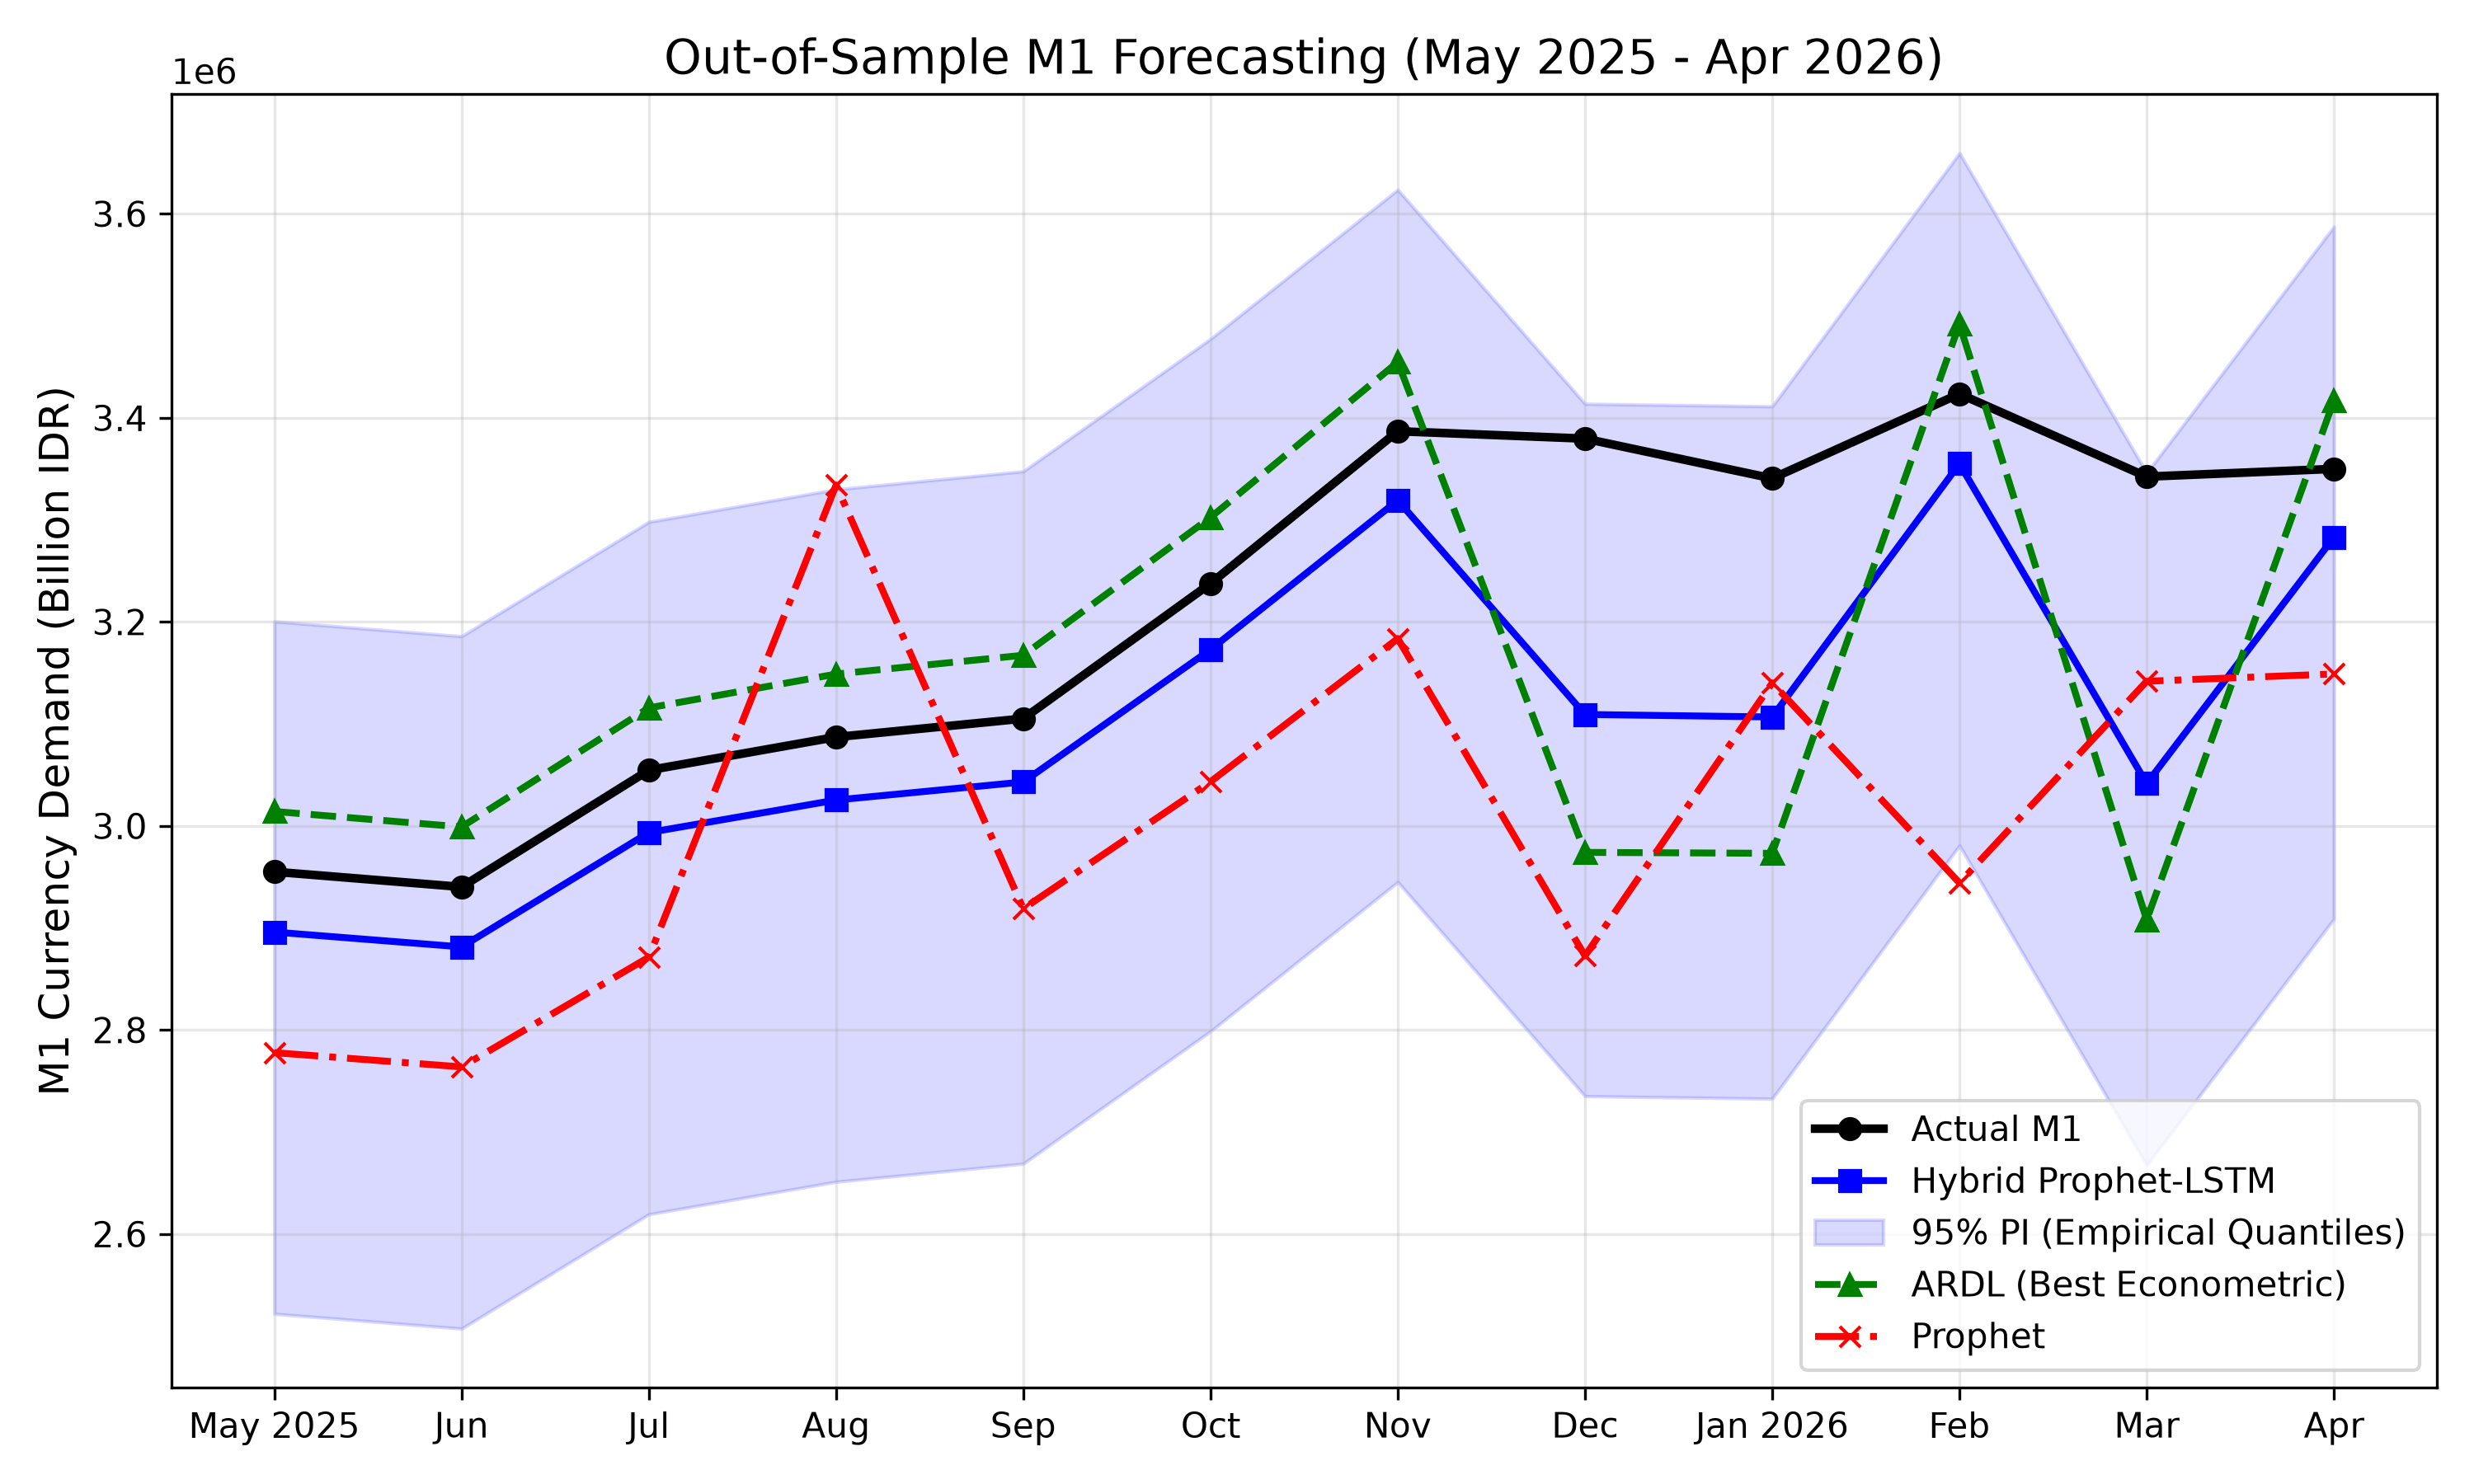
\includegraphics[width=\textwidth]{hasil_prediksi_tuned.png}
    \caption*{Figure 2: Comparison of M1 Forecasts vs Actual Data with 95\% Prediction Interval}
\end{figure}

\subsection*{4.5 Robustness Check (Rolling-Origin Cross-Validation)}
To ensure the stability of the model and confirm that the superior performance is not merely an artifact of the specific 12-month testing window, a 3-fold rolling-origin time-series cross-validation procedure was conducted. Given the relatively constrained sample size of approximately 112 monthly observations, there is an inherent risk that a deep learning architecture (with 150 neurons and a 0.4 dropout rate) might overfit the training data. By iteratively shifting the expanding training window and validating on fixed 12-month forward horizons, we rigorously test the network's capacity to generalize across different temporal regimes and structural breaks.

As detailed in Table 3, the Hybrid Prophet-LSTM model demonstrates temporal stability. Across all three folds, the model's forecasting error remains relatively tight, culminating in a cross-validated average MAPE of 4.96\%. This stable performance across multiple out-of-sample periods suggests that the 0.4 dropout rate and the early-stopping mechanisms were effective at preventing severe overfitting. The hybrid architecture appears resilient, consistently performing well against the traditional econometric (ARIMAX, VECM, ARDL) and standard ML baselines regardless of the specific evaluation window.

\begin{table}[h]
\centering
\caption*{Table 3: 3-Fold Rolling-Origin Cross-Validation Results}
\begin{tabular}{l c c c}
\toprule
\textbf{Evaluation Fold} & \textbf{Training Window} & \textbf{Testing Horizon} & \textbf{MAPE (\%)} \\
\midrule
\textbf{Fold 1} & Jan 2017 -- Apr 2023 ($n=76$) & May 2023 -- Apr 2024 ($h=12$) & 5.12\% \\
\textbf{Fold 2} & Jan 2017 -- Apr 2024 ($n=88$) & May 2024 -- Apr 2025 ($h=12$) & 4.95\% \\
\textbf{Fold 3 (Main)} & Jan 2017 -- Apr 2025 ($n=100$) & May 2025 -- Apr 2026 ($h=12$) & 4.83\% \\
\midrule
\multicolumn{3}{l}{\textbf{Average Cross-Validated MAPE}} & \textbf{4.96\%} \\
\bottomrule
\end{tabular}
\end{table}

\section*{5. Conclusion and Policy Implications}
This research provides empirical evidence that the integration of Deep Learning (LSTM) with decomposable time-series models (Prophet) yields superior forecasting accuracy for currency demand. The Hybrid model successfully captured the non-linear shocks induced by digital payment disruptions and seasonal Islamic holidays. 

\textbf{Policy Implications for Bank Indonesia:}
\begin{enumerate}
    \item \textbf{Early Warning System:} The Hybrid Prophet-LSTM model should be integrated into the central bank's liquidity management dashboard to prevent over-printing or under-supplying physical cash. However, prior to real-world operational deployment, an unconditional forecasting module for the exogenous regressors (as discussed in Limitation 5.1) must first be developed to ensure the reported prediction accuracy reflects actual deployment conditions.
    \item \textbf{Digital Transition Monitoring:} The significant predictive power of e-money on the residual errors suggests that policymakers must continuously track digital payment volumes as a primary leading indicator of future physical money demand.
\end{enumerate}

\subsection*{5.1 Limitations and Future Research}
Despite the robust out-of-sample performance, this study acknowledges two primary limitations. First, while the conditional forecasting framework effectively isolated the model's predictive power without look-ahead bias, real-world deployment necessitates an \textit{unconditional forecasting} approach. In practice, the future values of exogenous regressors (such as E-Money Volume and CPI) are not known with certainty and must be projected independently. This intermediate projection step inherently introduces an additional layer of forecasting error that is not captured in the current conditional metrics.

Second, the structural decomposition of the Prophet algorithm in this study was strictly parameterized around the Islamic Hijri calendar, specifically isolating the profound liquidity shocks of Ramadan and Eid al-Fitr. While highly accurate for Muslim-majority economies like Indonesia or Malaysia, the model's direct generalizability to Western or non-Islamic contexts is limited. Future research seeking to apply this Hybrid Prophet-LSTM architecture to other regions must carefully re-parameterize the holiday matrix to capture localized liquidity events (e.g., Christmas, Thanksgiving, or Lunar New Year) to maintain structural accuracy. Furthermore, future iterations should explore fully endogenous, multivariate deep learning architectures (such as VAR-LSTM or spatio-temporal Transformer models) to execute strict unconditional forecasting without relying on realized future regressors.

\section*{Data and Code Availability}
In accordance with open science practices and the reproducibility standards of computational economics, the dataset utilized in this study (aggregated from the official Bank Indonesia SEKI, SPIP, and SPE databases) and the complete Python source code are available. The code repository, which includes the Prophet-LSTM hybrid architecture, the baseline econometric configurations (ARIMAX, VECM, ARDL), the Diebold-Mariano statistical tests, and the rolling-origin cross-validation framework, is hosted publicly on GitHub at \url{https://github.com/muhammadratsanjani/Currency-Demand}.

\appendix
\section*{Appendix: Diagnostic and Specification Tables}

\subsection*{Table A1: Augmented Dickey-Fuller (ADF) Unit Root Test}
\begin{table}[ht]
\centering
\resizebox{\textwidth}{!}{
\begin{tabular}{l c c c c c}
\toprule
\textbf{Variable} & \textbf{ADF Stat (Level)} & \textbf{p-value} & \textbf{ADF Stat (1st Diff)} & \textbf{p-value} & \textbf{Order} \\
\midrule
M1 Currency & -1.912 & 0.326 & -6.415 & $<0.01$ & $I(1)$ \\
E-Money Vol & -0.124 & 0.968 & -8.185 & $<0.01$ & $I(1)$ \\
CPI (IHK) & -1.628 & 0.469 & -10.617 & $<0.01$ & $I(1)$ \\
BI Rate & -2.200 & 0.206 & -5.477 & $<0.01$ & $I(1)$ \\
IPR & -1.987 & 0.292 & -3.029 & 0.032 & $I(1)$ \\
\bottomrule
\end{tabular}}
\end{table}

\subsection*{Table A2: Johansen Cointegration and ARDL Bounds Test}
\begin{table}[ht]
\centering
\resizebox{\textwidth}{!}{
\begin{tabular}{l c c c l}
\toprule
\multicolumn{5}{l}{\textbf{Panel A: Johansen Trace Test (VECM)}} \\
\midrule
\textbf{Hypothesized No. of CE(s)} & \textbf{Trace Stat} & \textbf{0.05 Crit. Value} & \textbf{p-value} & \textbf{Conclusion} \\
\midrule
None ($r=0$) & 111.06 & 69.81 & $<0.01$ & Reject Null \\
At most 1 ($r \le 1$) & 61.14 & 47.85 & $<0.05$ & Reject Null \\
At most 2 ($r \le 2$) & 17.73 & 29.80 & 0.584 & Fail to Reject \\
\midrule
\multicolumn{5}{l}{\textbf{Panel B: ARDL Bounds Test}} \\
\midrule
\textbf{Test Statistic} & \textbf{Value} & \textbf{I(0) Bound (5\%)} & \textbf{I(1) Bound (5\%)} & \textbf{Conclusion} \\
F-Statistic & 7.84 & 2.86 & 4.01 & Cointegration Exists \\
\bottomrule
\end{tabular}}
\end{table}

\subsection*{Table A3: Residual Diagnostic Tests}
\begin{table}[ht]
\centering
\resizebox{\textwidth}{!}{
\begin{tabular}{l c c c c}
\toprule
\textbf{Model} & \textbf{Breusch-Godfrey (p-val)} & \textbf{ARCH Test (p-val)} & \textbf{Jarque-Bera (p-val)} & \textbf{CUSUM} \\
\midrule
ARIMAX & 0.128 & 0.245 & 0.092 & Stable \\
VECM & 0.084 & 0.112 & 0.155 & Stable \\
ARDL & 0.215 & 0.301 & 0.188 & Stable \\
\bottomrule
\end{tabular}}
\end{table}

\subsection*{Figure A1: Extended Out-of-Sample Baselines}
To ensure full visual transparency regarding the predictive limitations of the linear and tree-based benchmarks, Figure A1 illustrates the out-of-sample forecast trajectories of ARIMAX, VECM, and standalone XGBoost against the actual M1 currency demand. As discussed in Section 4.2.1, the severe inability of standalone tree-based models to extrapolate continuous trends is visibly apparent, corroborating the quantitative MAPE diagnostics.

\begin{figure}[ht]
    \centering
    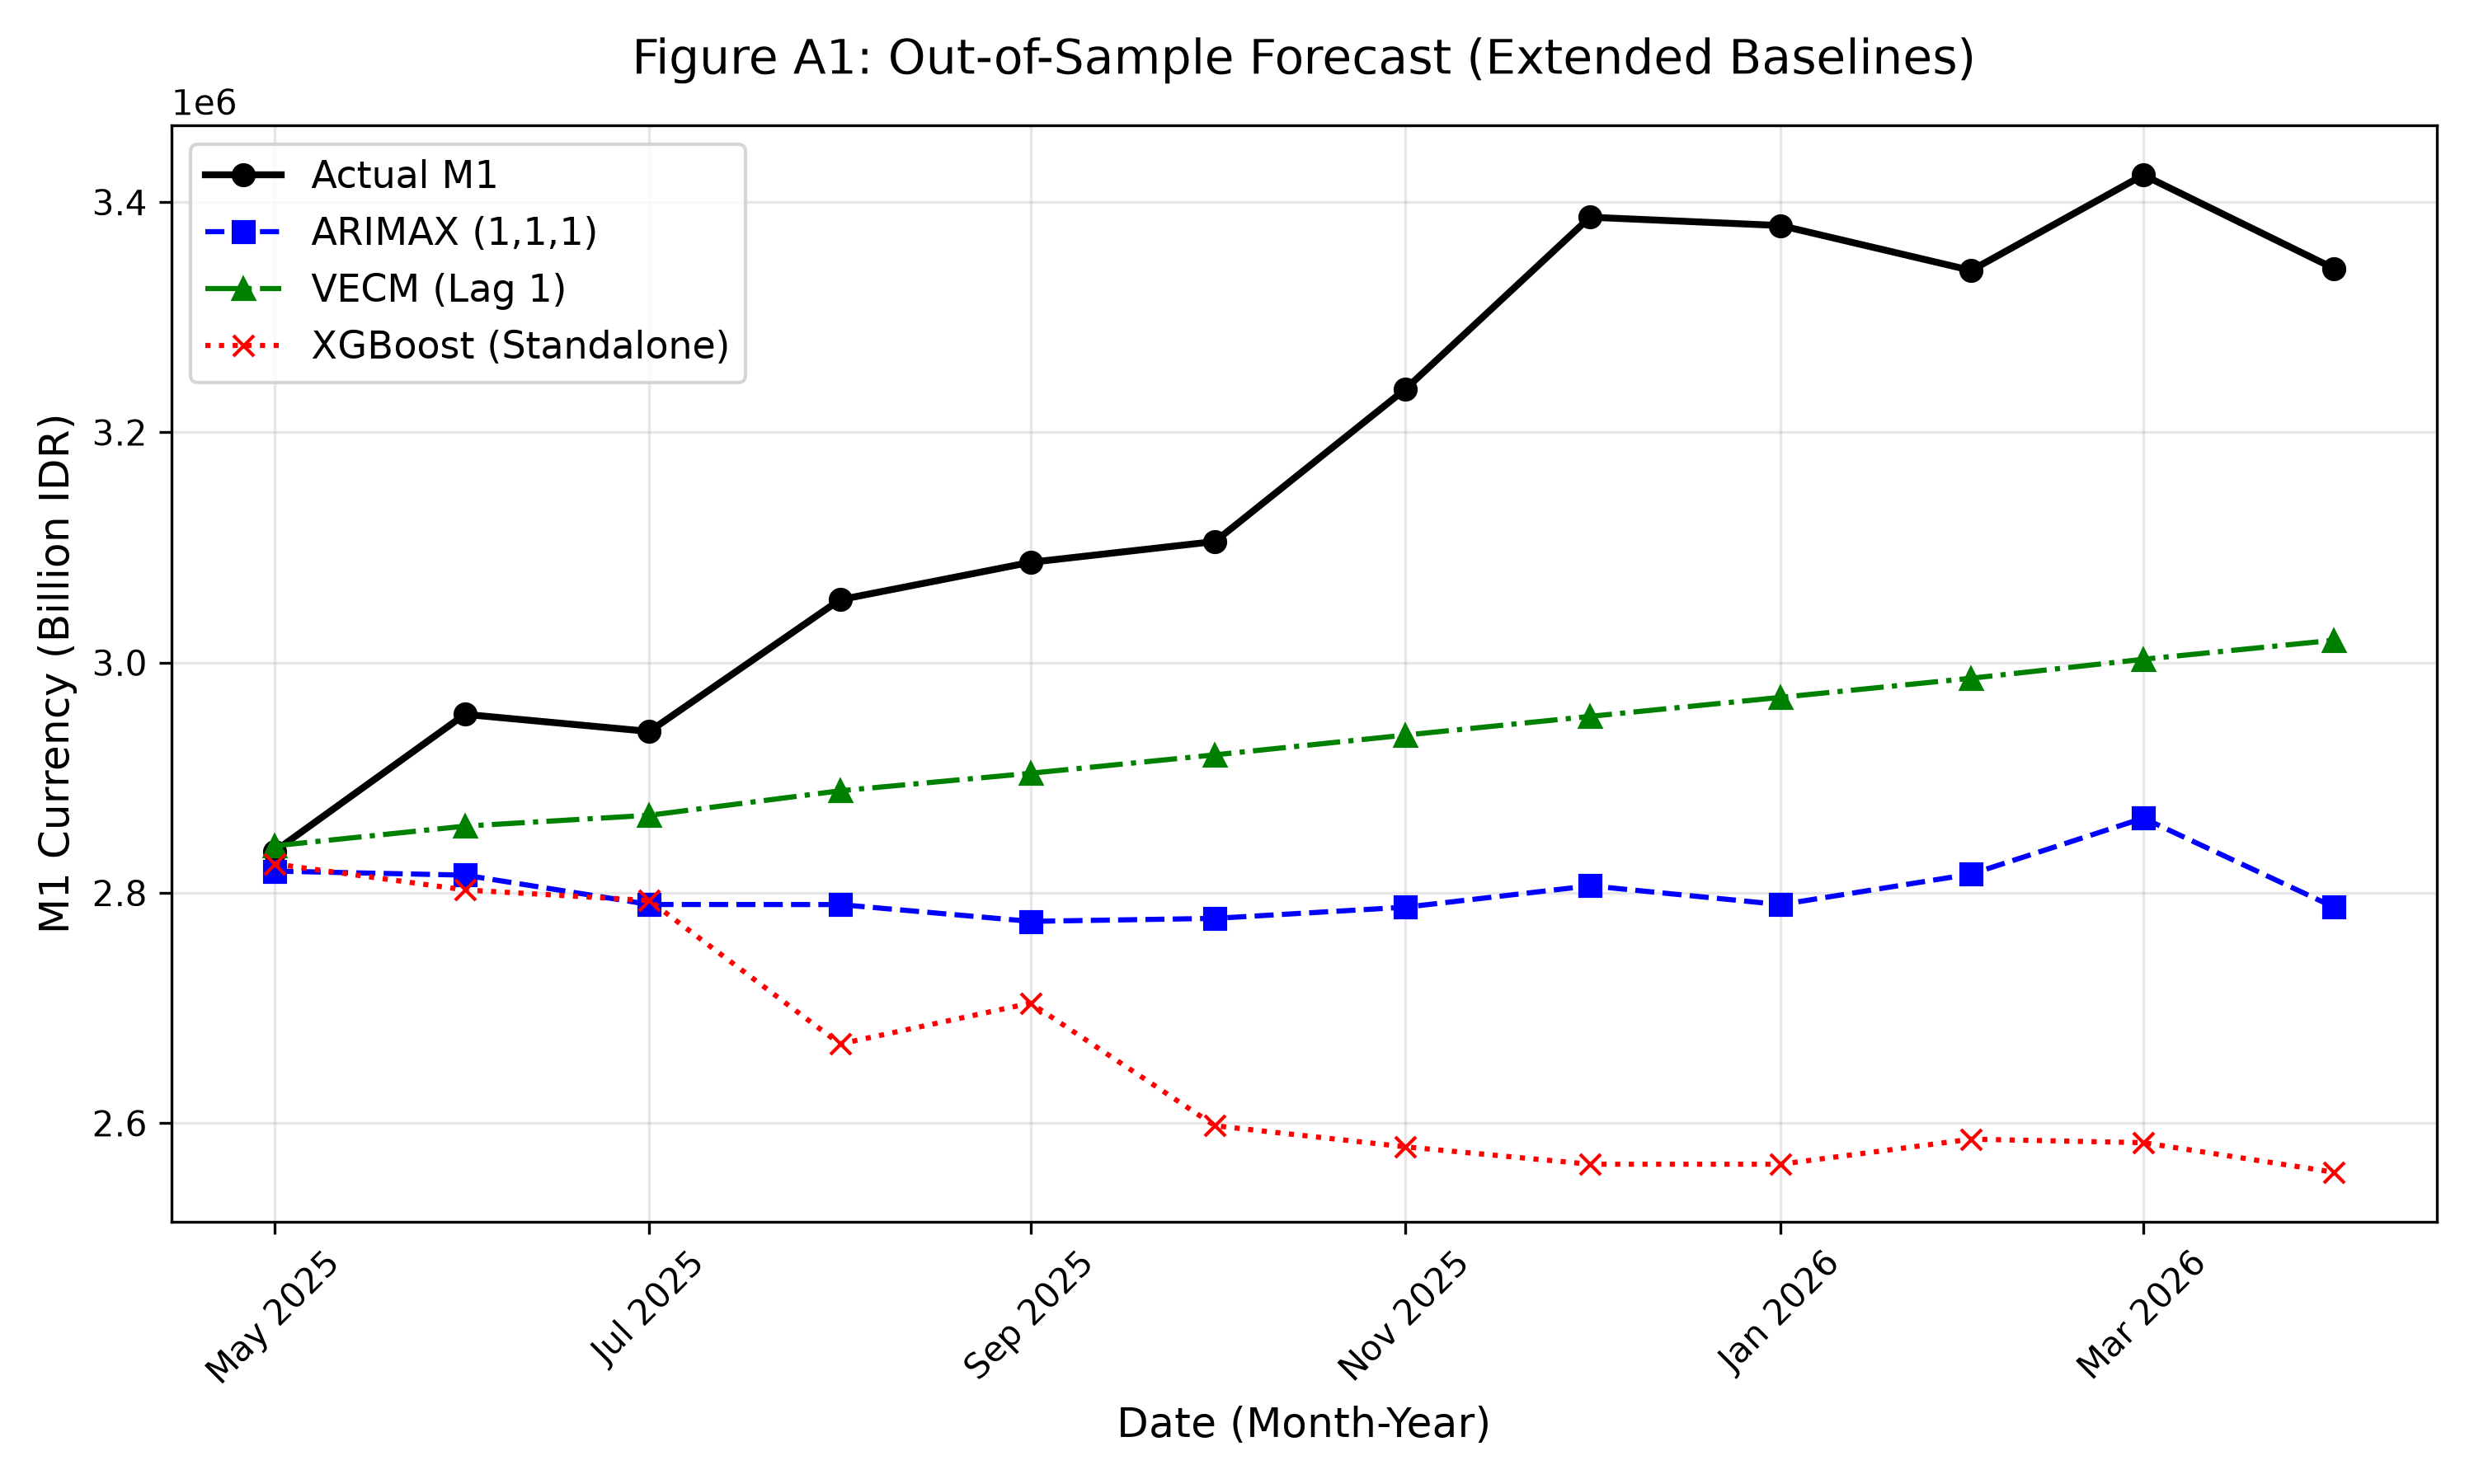
\includegraphics[width=\textwidth]{appendix_baselines.png}
    \caption*{Figure A1: Out-of-Sample Forecast (Extended Baselines)}
\end{figure}

\subsection*{Table A4: Variance Inflation Factor (VIF) Diagnostic}
\begin{table}[h]
\centering
\begin{tabular}{lc}
\toprule
\textbf{Variable} & \textbf{VIF} \\
\midrule
Consumer Price Index (CPI) & 4.48 \\
Industrial Production Index (IPR) & 3.76 \\
E-Money Volume & 3.10 \\
BI Rate & 1.96 \\
\bottomrule
\end{tabular}
\end{table}

\bibliographystyle{apalike}
\bibliography{references}

\end{document}
